% Partial resolution of Conjecture conj:gen (regression half): the bounded-drift
% knowability boundary. All numbers from scripts/regression_conjecture_validation.py
% (results/theory/regression_conjecture_validation.json).

This subsection resolves the regression half of Conjecture~\ref{conj:gen} for a natural
restricted family: \emph{bounded concept drift}. Two results: the adapt/freeze decision
is invariant to arbitrary unknown zero-mean label noise (where cardinal risk estimation
is confounded), and within drifts of known radius $B$ the knowability of $\sign\Delta$
admits a \emph{complete characterization} --- an exact, observable boundary.

\begin{theorem}[Noise-invariance of the regression decision]\label{thm:reg-noise}
Let $Y=g(X)+\epsilon$ with $\E[\epsilon\mid X]=0$ and arbitrary, unknown
(heteroscedastic) noise law. Under squared loss,
$\Delta=R_T(f_0)-R_T(f_a)=\E_T[(f_0-g)^2-(f_a-g)^2]$ does not depend on the noise,
while each absolute risk is shifted by the unidentifiable constant $\E[\epsilon^2]$.
The decision is ordinal-robust; cardinal risk estimation is confounded.
\end{theorem}
\begin{proof}
$R_T(f)=\E(f-g-\epsilon)^2=\E(f-g)^2+\E[\epsilon^2]$, the cross term vanishing by
$\E[\epsilon\mid X]=0$. The noise term cancels in the difference and survives in the
levels.
\end{proof}

\begin{theorem}[Bounded-drift knowability boundary; exact characterization]\label{thm:reg-iff}
Let the target conditional mean be $g_T=g_S+b$ with $\|b\|_\infty\le B$ for a known
radius $B$ (and the covariate-shift machinery of Theorem~\ref{thm:pos} available for the
source-transfer term). Define
\[
U=\E_T\!\big[(f_0-f_a)(f_0+f_a)\big],\qquad
T_S=\E_T\!\big[(f_0-f_a)\,g_S\big],\qquad
W=\E_T\!\big[|f_0-f_a|\big],
\]
where $U,W$ are computable from unlabeled target data and $T_S$ is importance-weighted
estimable from labeled source data with radius $\varepsilon_n$. Then
$\Delta=U-2T_S-2\,\E_T[(f_0-f_a)\,b]$ and $\big|\E_T[(f_0-f_a)\,b]\big|\le B\,W$, with
equality at the admissible drift $b^\star=-B\,\sign(f_0-f_a)$. Consequently, within the
family $\{\|b\|_\infty\le B\}$:
\begin{itemize}
\item[\textup{(i)}] \textup{(Achievability.)} The rule ``commit $\sign(U-2\widehat T_S)$
iff $|U-2\widehat T_S|>2BW+2\varepsilon_n$'' wrong-commits with probability at most
$\alpha$ against \emph{every} admissible drift, and its slack is unimprovable:
$b^\star$ attains it.
\item[\textup{(ii)}] \textup{(Converse.)} If $|U-2T_S|<2BW$, the reachable drift terms
fill $[-BW,\,BW]$ (scale $t\,b^\star$, $t\in[-1,1]$), so two admissible drifts give
$\Delta$ of opposite signs while all observables --- unlabeled target data and the
labeled source --- are unchanged. The pair realizes Theorem~\ref{thm:imp} inside the
family: the regime is unknowable.
\end{itemize}
Hence $\sign\Delta$ is label-free identifiable in the bounded-drift family \emph{if and
only if} $|U-2T_S|>2BW$: an exact knowability boundary, computable from observables, at
drift radius $B^\star=|U-2T_S|/(2W)$.
\end{theorem}
\begin{proof}
Expanding the squared losses, $\delta=(f_0-f_a)(f_0+f_a-2Y)$ and taking target
expectations with $Y=g_S+b+\epsilon$ (noise vanishing by
Theorem~\ref{thm:reg-noise}) gives the displayed decomposition. H\"older yields
$|\E_T[(f_0-f_a)b]|\le \|b\|_\infty\,\E_T|f_0-f_a|\le BW$, with equality iff
$b=-B\sign(f_0-f_a)$ a.e.\ on $\{f_0\ne f_a\}$ --- an admissible member of the family,
so the bracket is tight. (i): on the $1-\alpha$ event
$|\widehat T_S-T_S|\le\varepsilon_n$, the committed sign matches
$\sign(U-2T_S)$ and $|U-2T_S|>2BW$, so no admissible drift can flip $\Delta$.
(ii): the map $t\mapsto\E_T[(f_0-f_a)\,t\,b^\star]=-tBW$ is continuous and onto
$[-BW,BW]$; pick $t_\pm$ so that $\Delta(t_\pm)=U-2T_S+2t_\pm BW$ has opposite signs.
Since $b$ enters only through the target labels, neither the unlabeled target evidence
nor the source sample distinguishes the two worlds; apply Theorem~\ref{thm:imp}.
\end{proof}

\noindent\emph{Numerically validated}
(\texttt{regression\_conjecture\_validation.py}; Fig.~\ref{fig:regboundary}).
Across unknown noise scales $0\!\to\!2$, $\Delta$ is constant and the sign preserved
while the absolute risks drift apart (REG-1). Across drift radii
$B\in\{0,\dots,1.2\}$ with $40$ drifts per radius \emph{including the adversarial}
$b^\star$: zero false certifications at every radius; the adversarial drift saturates
the bracket to within $10^{-2}$ (tightness); the observable boundary evaluates to
$B^\star=0.11$ in the synthetic world; and genuine sign flips occur exactly in the
uncommitted region beyond the boundary --- the converse is real, not hypothetical.

\begin{figure}[t]\centering
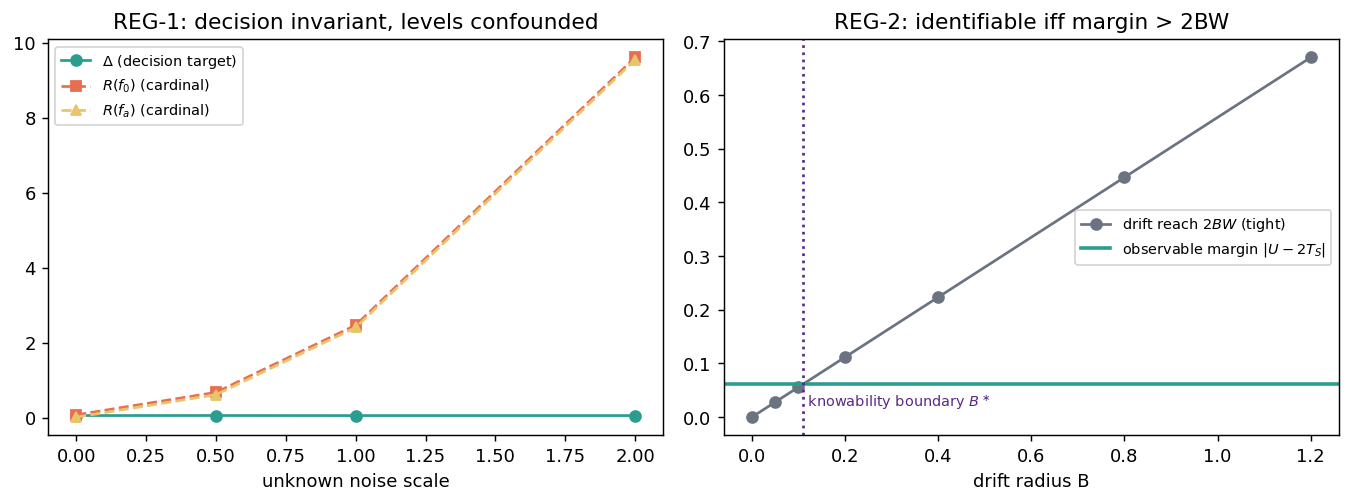
\includegraphics[width=0.92\textwidth]{figures/fig_regression_boundary.png}
\caption{The bounded-drift knowability boundary (Theorem~\ref{thm:reg-iff}). Left:
the decision target $\Delta$ is invariant to unknown label noise while cardinal risks
are confounded (Theorem~\ref{thm:reg-noise}). Right: identifiability holds exactly
while the observable margin $|U-2T_S|$ exceeds the tight drift reach $2BW$; the
crossing defines the computable boundary $B^\star$.}
\label{fig:regboundary}
\end{figure}

\paragraph{Weight (honest).} Theorem~\ref{thm:reg-iff} is, to our knowledge, the first
\emph{complete} per-family characterization in this paper beyond pure covariate shift:
both directions are proved and the boundary is computable from observables. Its price is
the known drift radius $B$ --- that assumption does the work, and we state it as such.
It resolves the regression half of Conjecture~\ref{conj:gen} \emph{for bounded drift};
fully general drift remains open and is exactly the unknowable regime of
Theorem~\ref{thm:imp}. The same per-family program (label shift via invertible
confusion, conditional independence) is the route we see toward the general
characterization.
